% !TEX TS-program = pdflatexmk
\documentclass[12pt]{article}

% Layout.
\usepackage[top=1in, bottom=0.75in, left=1in, right=1in, headheight=1in, headsep=6pt]{geometry}

% Fonts.
\usepackage{mathptmx}
\usepackage[scaled=0.86]{helvet}
\renewcommand{\emph}[1]{\textsf{\textbf{#1}}}

% Misc packages.
\usepackage{amsmath,amssymb,latexsym}
\usepackage{graphicx}
\usepackage{array}
\usepackage{xcolor}
\usepackage{multicol}
\usepackage{tabularx,colortbl}
\usepackage{enumitem}
%to make tikz pics work
\usepackage{tikz,pgfplots}

\usepackage[colorlinks=true]{hyperref}

% Paragraph spacing
\parindent 0pt
\parskip 6pt plus 1pt
\def\tableindent{\hskip 0.5 in}
\def\ts{\hskip 1.5 em}

\usepackage{fancyhdr}
\pagestyle{fancy} 
\lhead{\large\sf\textbf{MATH F251 Calculus I}}
\rhead{\large\sf\textbf{Fall 2019}}
\chead{\large\sf\textbf{Quiz 1: SAMPLE A}}

\newcommand{\localhead}[1]{\par\smallskip\textbf{#1}\nobreak\\}%
\def\heading#1{\localhead{\large\emph{#1}}}
\def\subheading#1{\localhead{\emph{#1}}}

\newenvironment{clist}%
{\bgroup\parskip 0pt\begin{list}{$\bullet$}{\partopsep 4pt\topsep 0pt\itemsep -2pt}}%
{\end{list}\egroup}%

\usetikzlibrary{calc}
\pgfplotsset{my style/.append style={axis x line=middle, axis y line=
middle, xlabel={$x$}, ylabel={$y$}, axis equal }}

\begin{document}
\textbf{Directions:} The quiz contains 20 problems. Place your answer in the blank provided. For graphing questions, a set of axes are provided. All graphs must be labeled.
\begin{enumerate}
%%%%
%type: numerical simplification
%%%%
\item Simplify ${\large{16^{-\frac{3}{4}}}}.$

\quad \hfill \underline{\hspace{2in}}
\vfill

\item Simplify ${\large{\log_{10}{0.001}}}.$

\quad \hfill \underline{\hspace{2in}}
\vfill

\item Find the exact value of $\cos ( 7 \pi /6).$

\quad \hfill \underline{\hspace{2in}}
\vfill

%%%%
%type: equation of a line
%%%%
\item Write the equation of the line between the points $(1,5)$ and $(-2,3)$ in the $y$-intercept form: $y=mx+b.$\\

\quad \hfill \underline{\hspace{2in}}
\vfill

%%%%
%type: simplification with exponent rules
%%%%
\item  Simplify the expression $\Large{\displaystyle{\left(\frac{3x^{\frac{1}{2}}y^5}{xy^2} \right)^2}}$. Write your answer without negative exponents.\\
\quad \\

\quad \hfill \underline{\hspace{2in}}
\vfill

%%%%%%%
%type: Questions from picture
\item Use the graph of $f(x)$ below to estimate the value of $x$ such that $f(x)=0.$
%Use the graph of $f(x)$ below to estimate $f(4).$ 

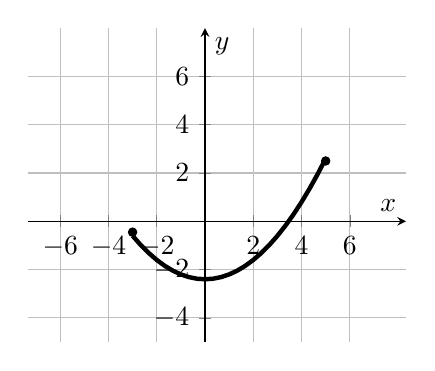
\begin{tikzpicture}
\begin{axis}[scale=.7, my style, xtick={-6,-4,-2,2,4,6}, ytick={-4,-2,2,4,6},
xmin=-4, xmax=5, ymin=-5, ymax=8,  
mark size=3.0pt, grid]
\addplot[domain=-3:5,ultra thick] {0.2*((x)^2)-2.4};
\addplot[mark=*,mark size=1.5,only marks] coordinates {(-3,-0.45)(5,2.5)};
\end{axis}
\end{tikzpicture}
\quad \hfill \underline{\hspace{2in}}
\newpage

%%%%
%type: expand and simplify
%%%%
\item Expand and simplify $3(x-6)-2(x^2-1).$

\quad \hfill \underline{\hspace{2in}}
\vfill

%%%%%%%
%type: solve an equation -- quadratic
\item Solve the equation $x^2=x+20.$
%Solve the equation $3x^2-2x-1=0.$

\quad \hfill \underline{\hspace{2in}}
\vfill
%%%%%%%
%type: piecewise defined function
\item Given the piecewise defined function below, determine the value(s) of $x$ such that $f(x)=4.$

$f(x)=\begin{cases} x^2 & x \leq 1 \\ x+1 & x >1 \end{cases}.$\\

\quad \hfill \underline{\hspace{2in}}
\vfill

%%%%%%%%%%
%type: misc
\item Determine where the graphs of $y=2x-1$ and $y=\sqrt{x}$ intersect.\\


\quad \hfill \underline{\hspace{2in}}
\vfill

%%%%%%%
%type: Difference quotient
\item For the function $f(x)=\frac{1}{x}$, find the expression $f(3)-f(3+h).$ Simplify your answer if possible.\\


\quad \hfill \underline{\hspace{2in}}
\vfill
\newpage
%%%%%%%%%%%%%
%type: inverse
\item Evaluate $\sin^{-1}(\frac{-1}{2}).$
%$h(x)=\frac{3}{x+1}.$

\quad \hfill \underline{\hspace{2in}}
\vfill

%%%%%%%%
%type: composition of functions
\item Given $f(x)=2x^2+x$ and $g(x)=e^x$, find $(f \circ g)(x).$ You do not need to simplify your answer.\\ \quad \\
%$f(x)=x-\sin x$ and $g(x)=x+1$

\quad \hfill \underline{\hspace{2in}}
\vfill


%%%%%%%%%
%type: exponential or log
\item Solve for $x$ in the equation $1+e^{2-x}=4.$
%$\ln ( x^2-5)=4$

\quad \hfill \underline{\hspace{2in}}
\vfill

%%%%%%
%Domain problems
%%%%%%%%
%type: domain roots
\item Determine the domain of $f(x)=\sqrt{2-4x}.$ Give your answer in interval notation.
%%$f(x)=\frac{1}{1-\sqrt[3]{x}}.$

\quad \hfill \underline{\hspace{2in}}
\vfill

%%%%%%%
%type: trig function
\item Solve for $\theta$ in the equation $\cos (\theta)=1.$
%$g(x)=\tan x.$


\quad \hfill \underline{\hspace{2in}}
\vfill
%%%%%%%
%%type: exponential or log
%\item Solve the inequality  $x^2 \geq 5x$ and give your answer in interval form.\\ \quad \\
%
%\quad \hfill \underline{\hspace{2in}}
%\vfill

\newpage
%%%%%%%%%
%Sketching Problems
%%%%%%%%%
Graph the following functions. Identify and label any asymptotes, $x$- or $y$-intercepts.
%type: graph 1/x
\begin{multicols}{2}{
      % make sure you added \usepackage{enumerate}
      \vspace*{-0.45in}
%      \begin{enumerate}[(a)]
      \item $f(x) =\frac{1}{x^2}$

\begin{tikzpicture}[scale=0.6][>=latex]
%x axis
\draw[->] (-5 ,0) -- (5 ,0) node[below] {$x$};
\foreach \x in {-4,...,4}
\draw[shift={(\x,0)}] (0pt,2pt) -- (0pt,-2pt);
%y axis
\draw[->] (0,-5) -- (0,5) node[left] {$y$};
\foreach \y in {-4,...,4}
\draw[shift={(0,\y)}] (2pt,0pt) -- (-2pt,0pt);
%\node[below left] at (0,0) {\footnotesize $0$};
\end{tikzpicture}
 
 \item $f(x) = 1+e^{-x} $ 

\begin{tikzpicture}[scale=0.6][>=latex]
%x axis
\draw[->] (-5 ,0) -- (5 ,0) node[below] {$x$};
\foreach \x in {-4,...,4}
\draw[shift={(\x,0)}] (0pt,2pt) -- (0pt,-2pt);
%y axis
\draw[->] (0,-5) -- (0,5) node[left] {$y$};
\foreach \y in {-4,...,4}
\draw[shift={(0,\y)}] (2pt,0pt) -- (-2pt,0pt);
\end{tikzpicture}
}
\end{multicols}

\vfill 
%\begin{multicols}{2}{
      % make sure you added \usepackage{enumerate}
      \vspace*{-0.45in}
%      \begin{enumerate}[(a)]
      \item $f(x) =\cos(2x)$ on the interval $[-2\pi, 2\pi]$

\begin{tikzpicture}[scale=0.6][>=latex]
%x axis
\draw[->] (-5 ,0) -- (5 ,0) node[below] {$x$};
\foreach \x in {-4,...,4}
\draw[shift={(\x,0)}] (0pt,2pt) -- (0pt,-2pt);
%y axis
\draw[->] (0,-5) -- (0,5) node[left] {$y$};
\foreach \y in {-4,...,4}
\draw[shift={(0,\y)}] (2pt,0pt) -- (-2pt,0pt);
%\node[below left] at (0,0) {\footnotesize $0$};
\end{tikzpicture}
 \vfill
 \item Use triangles to determine $\tan \theta$ assuming $\sin \theta = \frac{1}{3}$ and $\theta$ is in the first quadrant. \\ \quad \\
 
\quad \hfill \underline{\hspace{2in}}
\vfill

\vspace{1.3in}

\end{enumerate}
\end{document}
